\documentclass[utf8]{FrontiersinVancouver}

\usepackage{url,hyperref,lineno,microtype,setspace}
\usepackage{booktabs}
\usepackage{tabularx}
\usepackage{longtable}
\usepackage{float}
\usepackage{xcolor}
\usepackage{graphicx}
\graphicspath{{./}}
\setkeys{Gin}{width=\textwidth,keepaspectratio}
\linenumbers
\setcitestyle{square,numbers}
\emergencystretch=2em

\def\keyFont{\fontsize{8}{11}\helveticabold}
\def\firstAuthorLast{Liu {et~al.}}
\def\Authors{Cuicui Liu\,$^{1,*}$, Huan Peng\,$^{2}$ and Shuang Wu\,$^{3,*}$}
\def\Address{$^{1}$College of Information Engineering, Changsha Medical University, Changsha 410219, Hunan, China \\
$^{2}$School of Computer Science and Technology, Changsha University of Science and Technology, Changsha, Hunan, China \\
$^{3}$The Affiliated Changsha Central Hospital, Hengyang Medical School, University of South China, Changsha 410004, Hunan, China}
\def\corrAuthor{Cuicui Liu and Shuang Wu}
\def\corrEmail{\nolinkurl{liucuicui@csmu.edu.cn}, \nolinkurl{2018051139@usc.edu.cn}}
\newcommand{\TOM}{TOM500}
\newcommand{\TAO}{thyroid-associated ophthalmopathy}
\newcommand{\CAS}{Clinical Activity Score}
\newcommand{\ari}{adjusted Rand index}

\begin{document}
\onecolumn
\firstpage{1}

\title[Orbital MRI phenotyping in thyroid-associated ophthalmopathy]{Volume-Based Multi-Tissue Orbital MRI Phenotyping in Thyroid-Associated Ophthalmopathy: Reproducibility and Exploratory Associations With the Clinical Activity Score}
\author[\firstAuthorLast]{\Authors}
\address{}
\correspondance{}
\extraAuth{}
\maketitle

\begin{abstract}
\textbf{Background:} Thyroid-associated ophthalmopathy (TAO) has heterogeneous orbital tissue involvement, whereas the Clinical Activity Score (CAS) summarizes activity from clinical findings. Whether orbital MRI morphology yields reproducible phenotypes is unclear. \textbf{Objective:} To identify reproducible volume-based MRI phenotypes and characterize their exploratory associations with CAS. \textbf{Methods:} We analyzed 500 TOM500 cases. Nine annotated structures were represented by physical volumes and compositional fractions. K-means clustering was fitted in 400 training cases, and frozen centroids were assigned to 100 validation cases. Stability was evaluated with 1,000 bootstrap resamples using the adjusted Rand index (ARI). CAS was analyzed before and after adjustment for age, sex, smoking index, and disease duration. \textbf{Results:} The three-cluster solution had a training bootstrap ARI of 0.862 $\pm$ 0.103. Unadjusted CAS distributions differed in training ($P=2.27\times10^{-9}$) and validation ($P=4.01\times10^{-4}$). Leave-one-tissue solutions retained similarity to the primary solution (ARI 0.653--0.925), whereas single-tissue solutions did not (ARI 0.036--0.316). After adjustment, continuous CAS remained associated in training ($P=2.09\times10^{-7}$), but validation evidence was inconsistent, with nominal support for continuous CAS ($P=0.0495$) and no support for CAS $\geq 3$ ($P=0.543$). \textbf{Conclusions:} Volume-based multi-tissue MRI features provide a reproducible exploratory representation of TAO heterogeneity and an auditable basis for CAS-linked endocrine-imaging research.
\end{abstract}

\tiny
\keyFont{\section{Keywords:} thyroid-associated ophthalmopathy, thyroid eye disease, orbital magnetic resonance imaging, multi-tissue phenotype, volume-based phenotyping, unsupervised clustering, Clinical Activity Score, reproducibility}

\section{Introduction}
\TAO, also called thyroid eye disease or Graves' orbitopathy, is an autoimmune orbital disorder with heterogeneous tissue involvement and variable clinical activity. The extraocular muscles, orbital fat, lacrimal gland, optic nerve, and adjacent orbital structures may be affected in different combinations, and these tissues do not necessarily change in parallel \citep{bahn2010,taylor2020}. This heterogeneity is clinically relevant because active disease and residual structural disease can require different management approaches \citep{bartalena2021,douglas2020}. Treatment-related changes in extraocular muscle and orbital fat volume further illustrate why tissue-level measurements may complement clinical assessment \citep{jain2022}. The Clinical Activity Score (CAS) is widely used to summarize inflammatory activity, but it captures a limited set of clinical signs rather than the spatial distribution and relative burden of orbital tissue involvement \citep{mourits1997}. A patient-level imaging phenotype could therefore provide a complementary description of TAO heterogeneity if its reproducibility and relationship with CAS are established transparently.

Orbital MRI provides the anatomic coverage and quantitative information needed to study this problem. Earlier MRI studies examined extraocular-muscle involvement and relationships between imaging findings and clinical activity, including in patients with prolonged disease duration \citep{yokoyama2002,tortora2013,zhou2019,huo2022}. Quantitative MRI and radiomics have since expanded the measurable feature space beyond visual assessment \citep{zhang2024,wang2025,lambin2012,gillies2016,yip2016}. Radiomics studies in other organs have also shown that MRI or CT texture and multivariable feature representations can support diagnostic or prognostic modeling, but their reproducibility depends on acquisition, segmentation, preprocessing, and feature-definition choices \citep{yi2018adrenal,yang2025mri,he2025prior}. Recent supervised studies have used whole-orbit or multi-region radiomics to predict intravenous glucocorticoid response, and multimodal models have combined MRI features with clinical variables for the same endpoint \citep{zhang2024response,zhou2026response}. These studies show that different orbital regions can provide complementary information, but their predefined clinical outcomes do not establish whether the underlying multi-tissue morphology forms reproducible patient-level phenotypes before clinical labels are used.

The unresolved question is therefore a reproducibility question rather than a simple cluster-separation question. A volume-based phenotype should remain reasonably stable under patient-level resampling, alternative feature representations, and scaling choices. Radiomics reporting recommendations emphasize standardized feature definitions and transparent processing because apparently predictive features can be sensitive to implementation details \citep{zwanenburg2020,vangriethuysen2017}. If the phenotype is genuinely multi-tissue, removing one annotated structure should not eliminate the overall organization, whereas a single-tissue solution should not reproduce the complete pattern. A fixed validation partition can further test whether training-derived centroids can be assigned to new cases without refitting the clusters. Cluster separation and agreement should be interpreted with complementary measures, including silhouette-based geometry and partition agreement metrics \citep{rousseeuw1987,hubert1985}. Clinical characterization then needs to distinguish an unadjusted CAS gradient from covariate-adjusted association, with age, sex, smoking index, and disease duration treated as potential sources of imbalance. This design links the imaging phenotype to a clinical endpoint while keeping reproducibility as the primary evidentiary target.

The TOM500 resource enables this analysis at the patient level. It contains 500 T2-weighted orbital MRI cases with masks for nine annotated orbital structures and a clinical table including CAS, age, sex, smoking index, and disease duration \citep{zhang2025tom500}. Tissue measurements can therefore be aggregated across the orbit without treating the two eyes from one patient as independent observations. The available clinical fields also define the scope of the endocrine-imaging question. CAS is used for clinical characterization, while the present analysis does not estimate associations with thyroid hormone concentrations, thyroid autoantibodies, proptosis, treatment exposure, or treatment response because those fields are not part of the verified table.

We performed a retrospective public-dataset analysis with three linked objectives. First, we tested whether physical volumes and compositional volume fractions from the nine annotated tissues yielded a reproducible volume-based multi-tissue phenotype in a fixed 400-case training partition, using bootstrap stability and feature-, scaling-, and tissue-sensitivity analyses. Resampling was used to quantify variability rather than to imply transportability to a new population \citep{efron1993}. Second, we assigned the frozen training-derived phenotype to a 100-case validation partition and characterized its CAS distribution. Third, we estimated covariate-adjusted associations with continuous CAS and an exploratory CAS threshold, preserving the distinction between training evidence and fixed-partition validation evidence. The resulting framework provides an auditable way to describe coordinated orbital MRI variation, evaluate its clinical relevance, and establish a reusable foundation for future endocrine-imaging studies of TAO heterogeneity.

\section{Materials and methods}
\subsection{Study design and data source}
This retrospective cross-sectional analysis used the public \TOM{} dataset and its companion clinical table \citep{zhang2025tom500}. The analysis was organized around a patient-level mapping from nine annotated orbital tissues to a low-dimensional volume-led phenotype, followed by fixed-centroid assignment and CAS characterization. Figure~\ref{fig:workflow} summarizes this information flow. The verified clinical fields were age, sex, smoking index, disease duration, and CAS. TSH, FT4, TRAb, proptosis, treatment exposure, and treatment response were not available in the analyzed table and were outside the study scope.

The dataset supplied a fixed 400-case training partition and a 100-case validation partition. Feature imputation, scaling, cluster fitting, and bootstrap resampling were performed within the training partition. The validation partition received only the frozen training-derived preprocessing parameters and cluster centroids. It was therefore treated as a fixed internal validation partition, not as an external cohort. All analysis units were patient-level cases, and no bilateral-eye observation was counted as an independent patient. The dataset was used under its public data-access and citation conditions, with no new patient contact or intervention.

\begin{figure}
  \centering
  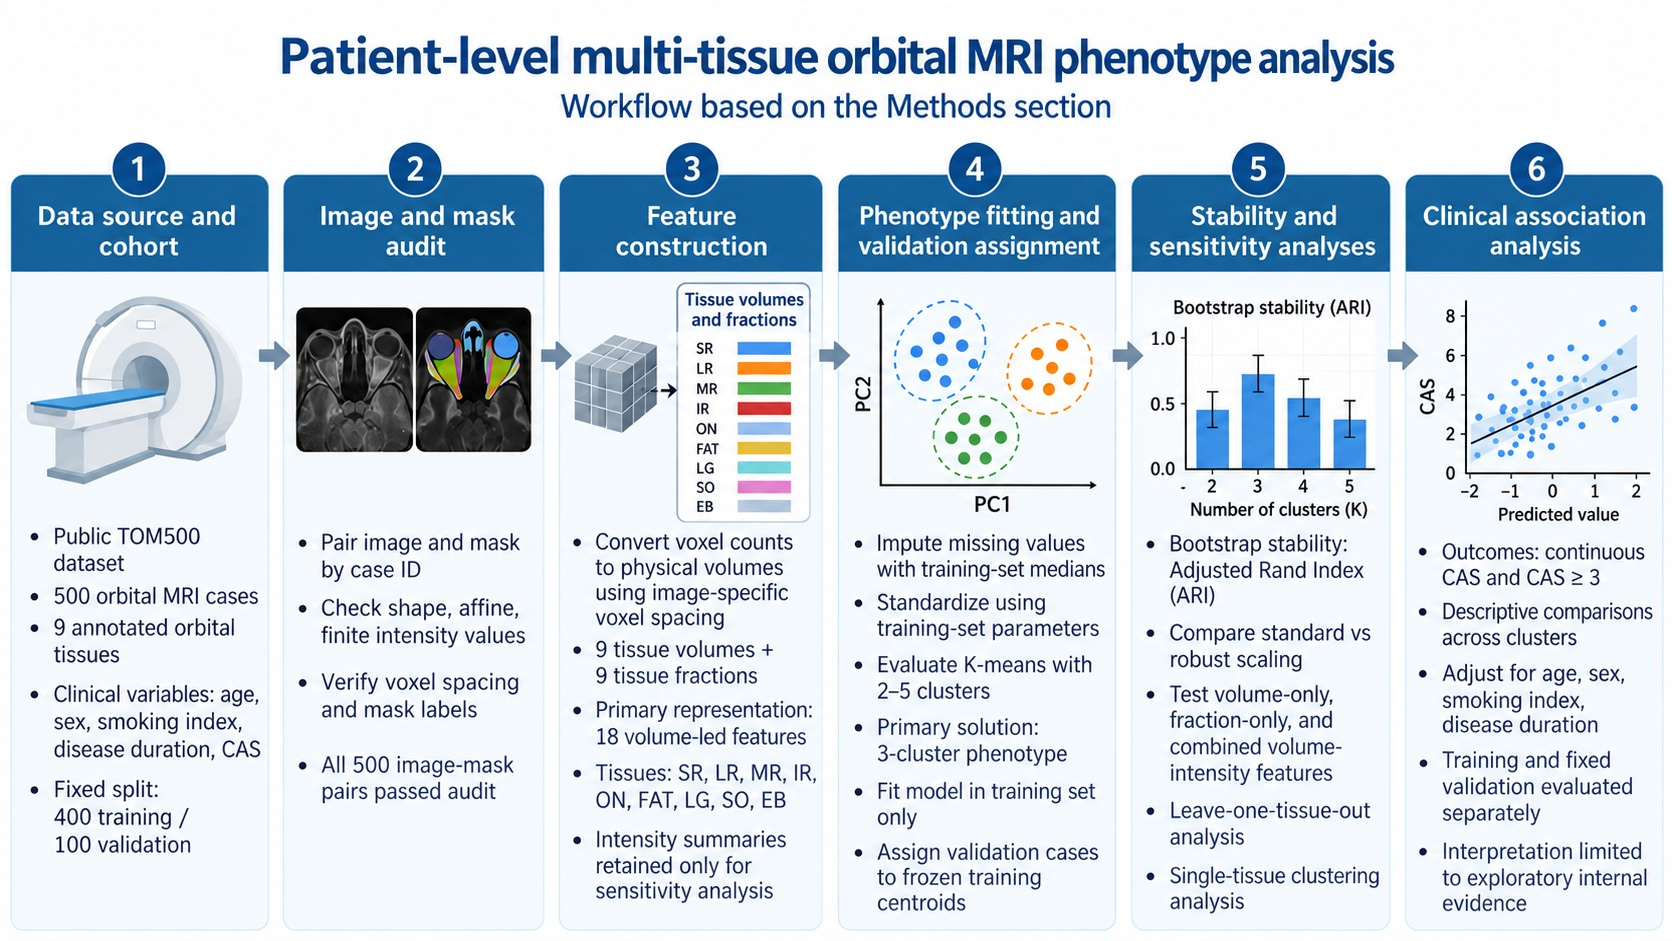
\includegraphics{Figure1_workflow.jpg}
  \caption{Study and analysis framework. Patient-level TOM500 MRI and mask pairs were audited before nine tissue volumes and compositional fractions were constructed. The volume-led representation was fitted in 400 training cases, assessed with stability and sensitivity analyses, and transferred to 100 fixed validation cases through frozen-centroid assignment. CAS analyses were performed separately in the training and validation partitions.}
  \label{fig:workflow}
\end{figure}

\subsection{Image and mask audit}
Each MRI volume was paired with the mask sharing its case identifier. The audit checked image and mask dimensions, affine information, finite intensities, voxel spacing, and the complete set of mask labels before feature extraction. This explicit image-mask audit follows the general requirement that segmentation and preprocessing be traceable in quantitative imaging studies \citep{zwanenburg2020,song2022mri}. All 500 image-mask pairs had dimensions $512\times512\times20$, and all ten mask values, including background and nine annotated labels, occurred in every case. The modal voxel spacing was $0.3125\times0.3125\times3.85$ mm in 467 of 500 cases, while the remaining scans showed small spacing deviations. Image-specific header spacing was therefore used to convert voxel counts to physical volumes, preserving the acquisition-specific geometry in the feature table.

\subsection{Feature construction}
For tissue $i$, the voxel count $n_i$ was converted to a physical volume using the voxel dimensions recorded in the corresponding image header:
\begin{equation}
V_i=n_i\,s_xs_ys_z,
\label{eq:volume}
\end{equation}
where $s_x$, $s_y$, and $s_z$ are the in-plane and through-plane voxel spacings in millimeters. Equation~\ref{eq:volume} converts each mask count into a case-specific physical measurement before tissue composition is calculated. The composition of the annotated orbital tissues was then represented by the fraction
\begin{equation}
f_i=\frac{V_i}{\sum_{j=1}^{9}V_j}, \qquad i=1,\ldots,9.
\label{eq:fraction}
\end{equation}
Thus, $V_i$ describes the physical burden of tissue $i$, while $f_i$ describes its share of the total volume represented by the nine annotated tissues. The denominator is not the number of nonzero MRI intensity voxels, so the fractions sum to one for each case. An audit of the legacy feature table found that its alternative denominator produced fractions summing to 0.0313--0.0632 across cases. Those legacy values were excluded from the corrected analysis, and the fractions in Eq.~\ref{eq:fraction} were used for clustering, sensitivity analyses, and association analyses.

The primary volume-led feature vector for each patient was
\begin{equation}
\boldsymbol{x}^{(V)}=\left[V_1,\ldots,V_9,f_1,\ldots,f_9\right]^{\mathsf{T}},
\label{eq:volume-feature-vector}
\end{equation}
which contained 18 variables. Equation~\ref{eq:volume-feature-vector} makes the two feature families explicit, with physical volumes followed by their corresponding tissue fractions. The nine structures were the superior rectus/levator complex (SR), lateral rectus (LR), medial rectus (MR), inferior rectus (IR), optic nerve (ON), orbital fat (FAT), lacrimal gland (LG), superior oblique (SO), and eyeball (EB), following the dataset documentation \citep{zhang2025tom500}.

The intensity sensitivity representation added three within-mask summaries for each tissue: mean, standard deviation, and 90th percentile. Before these summaries were calculated, each scan was centered by the median and scaled by the interquartile range of its finite, nonzero MRI voxels. When that interquartile range was non-positive, the image-wide standard deviation was used as the scale. This produced 27 intensity variables, or $9\times3$, and a 45-variable combined representation formed by concatenating the 18 volume-led variables with the 27 intensity variables. This restrained feature-family design was kept separate from higher-dimensional radiomics pipelines and multimodal image models reported in recent medical imaging studies \citep{wang2025bone,he2025histopath,li2023multimodal}. Related decision-support, segmentation, and glioma-analysis studies illustrate the broader use of machine learning in medical imaging, while addressing different tasks from the present phenotype analysis \citep{li2025edge,li2026kdlm,wu2025ffbformer}. Column-wise medians were estimated from the training partition for missing-value imputation. The imputed training matrix was then standardized with training-fitted parameters, and the same imputation values and scaling parameters were applied unchanged to validation cases.

\subsection{Phenotype fitting and fixed validation assignment}
The imputed and standardized feature matrix was denoted by $\widetilde{X}\in\mathbb{R}^{n\times p}$, where $n$ is the number of patient cases and $p$ is the number of features in the representation under evaluation. K-means models with two through five clusters were evaluated during the exploratory pilot. For a candidate number of clusters $K$, the training objective was the within-cluster squared Euclidean distance:
\begin{equation}
\min_{\{\boldsymbol{\mu}_k\},\{c_a\}}\sum_{a=1}^{n}\left\|\widetilde{\boldsymbol{x}}_a-\boldsymbol{\mu}_{c_a}\right\|_2^2,
\qquad c_a\in\{1,\ldots,K\},
\label{eq:kmeans}
\end{equation}
where $\widetilde{\boldsymbol{x}}_a$ is the standardized feature vector for case $a$, $c_a$ is its cluster assignment, and $\boldsymbol{\mu}_k$ is the centroid of cluster $k$. Equation~\ref{eq:kmeans} defines the unsupervised fitting step, whereas the stability-first rule determines which candidate value of $K$ is retained. Model selection ranked candidate solutions first by mean bootstrap ARI across 1,000 resampled training sets and then by training silhouette only if the bootstrap ARI means were exactly tied. The primary three-cluster volume-led solution was selected under this exploratory stability-first rule. This rule explains why the two-cluster solution was not retained solely because it had a higher single-partition silhouette.

The final model was fitted only in the training partition. For a validation feature vector $\widetilde{\boldsymbol{x}}$, assignment used the nearest frozen training centroid:
\begin{equation}
\widehat{c}(\widetilde{\boldsymbol{x}})=\underset{k\in\{1,\ldots,K\}}{\operatorname{argmin}}\left\|\widetilde{\boldsymbol{x}}-\boldsymbol{\mu}_k\right\|_2^2,
\label{eq:centroid-assignment}
\end{equation}
where $\boldsymbol{\mu}_k$ is the centroid estimated from the training cases. Validation cases were assigned with Eq.~\ref{eq:centroid-assignment} and were not used to refit centroids, preprocessing parameters, or cluster labels. The silhouette coefficient was calculated on the complete standardized training matrix and its fitted labels. Bootstrap stability was quantified by the adjusted Rand index (ARI) between the reference labels and labels obtained after refitting K-means to each resampled training matrix. Sensitivity ARI values compared labels from an alternative representation with the primary labels on the same training cases.

\subsection{Stability and sensitivity analyses}
Bootstrap stability was summarized with the ARI between the reference training labels and the labels generated from 1,000 resampled training sets. Each resample was analyzed with the same feature construction, training-partition imputation, scaling, and K-means fitting protocol. Sensitivity analyses compared standard scaling with robust scaling, physical-volume-only features, fraction-only features, and the 45-feature combined representation defined above. To assess whether the phenotype depended on one structure, the 18-feature representation was recalculated after removing each tissue and the three-cluster model was refitted. Separate three-cluster models were also fitted for each tissue. These comparisons evaluated representation stability, not biological independence or mechanistic specificity.

\subsection{Clinical association analysis}
CAS was analyzed in its observed ordinal range as a continuous score and as an exploratory binary endpoint defined by CAS $\geq3$. Cluster differences in continuous clinical variables were summarized with medians and interquartile ranges and compared with Kruskal--Wallis tests. Sex distributions were summarized with counts and percentages and compared with a chi-square test. Covariate-adjusted associations were estimated with heteroskedasticity-robust linear regression for continuous CAS and robust binomial logistic regression for CAS $\geq3$. The covariates were age, sex, smoking index, and disease duration, which were included because they differed across imaging clusters or were clinically relevant potential sources of imbalance. The adjusted models characterized association and potential confounding. They were not used to estimate a causal effect or treatment benefit.

As a sensitivity analysis, CAS was also modeled as an ordinal outcome using proportional-odds logistic regression across the observed CAS categories. This model used the same covariates, training-referenced covariate standardization, and frozen cluster assignments as the primary adjusted analyses. Proportional-odds adequacy was inspected by fitting threshold-specific binary logistic models. The highest CAS thresholds contained few events and some threshold-specific fits did not converge, so the inspection was treated as descriptive rather than as a definitive formal assumption test. Results from this sensitivity model were therefore interpreted alongside, and not in place of, the continuous and binary analyses.

\subsection{Reproducibility and claim boundary}
Numerical results were generated by the server-run analyses archived as evidence files. The analysis did not evaluate clinical utility, treatment response, prospective deployment, or causal mechanisms. The fixed 100-case partition was used to assess assignment of frozen training-derived phenotypes and was not treated as external validation. The available clinical table defined the endocrine-imaging scope: the analysis could characterize CAS-linked imaging patterns, but it could not test associations with thyroid hormone concentrations, thyroid autoantibodies, proptosis, or treatment outcomes.

\section{Results}
\subsection{Cohort and data integrity}
The analysis included 500 patient-level cases, comprising 400 training cases and 100 cases in the fixed validation partition. All 500 image-mask pairs passed the loading, shape, affine, intensity, spacing, and label checks, and every case identifier matched the clinical table. CAS values were distributed as 0:171, 1:128, 2:80, 3:67, 4:33, 5:17, and 6:4. Thus, the continuous score and the exploratory threshold CAS $\geq3$ represented the same patient-level endpoint at two resolutions, with 121 of 500 cases meeting the threshold. These audit results define the complete denominator for the phenotype and CAS analyses.

\subsection{Primary phenotype and cluster-number comparison}
The 18-feature volume-led representation, consisting of nine physical volumes and nine compositional fractions, produced training clusters of 148, 164, and 88 cases. Assignment of the frozen training centroids to the validation partition yielded 38, 35, and 27 cases, respectively. For the selected three-cluster solution, the training silhouette was 0.188 and the mean ARI across 1,000 bootstrap resamples was 0.862 $\pm$ 0.103. The two-cluster solution was geometrically more compact, with a silhouette of 0.272, which was 0.084 higher, but its bootstrap ARI was 0.844 $\pm$ 0.118, 0.019 lower than the three-cluster value. Four- and five-cluster solutions had still lower bootstrap ARI means of 0.531 and 0.544. The comparison therefore separates single-partition compactness from resampling reproducibility. Because the analysis rule ranked mean bootstrap ARI before silhouette, the three-cluster solution was retained as the primary reproducible representation, rather than being selected on silhouette alone.

The cluster profiles showed coordinated variation across the nine annotated orbital tissues rather than separation along a single measurement axis (Figure~\ref{fig:phenotype}). All subsequent validation and CAS analyses used this frozen partition. The reported clinical contrasts therefore reflect assignment to training-derived centroids, not clusters refitted after the validation outcomes were available.

\begin{figure}
  \centering
  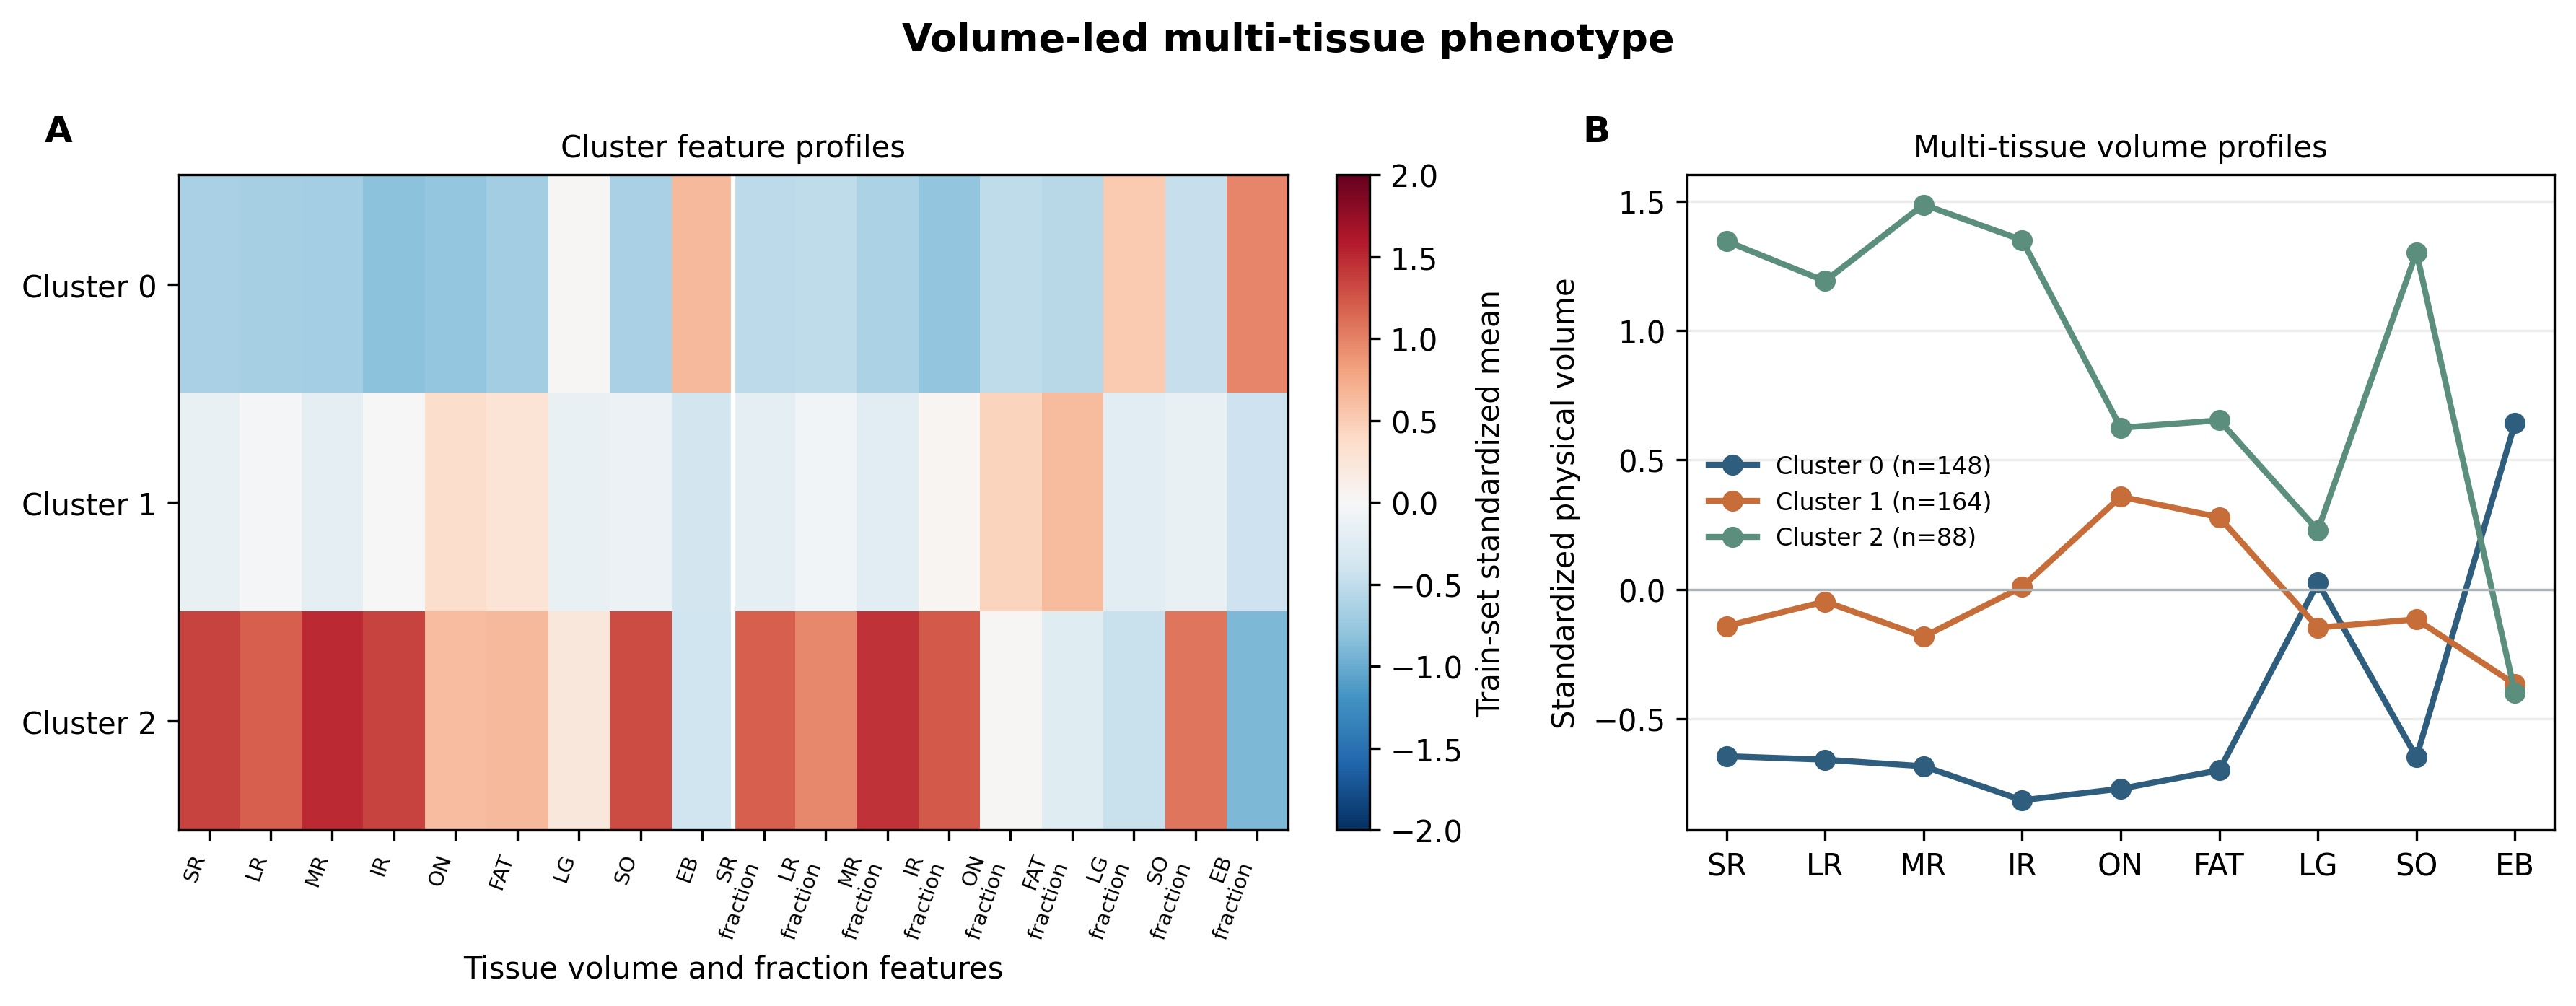
\includegraphics{Figure2_phenotype_profiles.jpg}
  \caption{Multi-tissue phenotype profiles. The primary representation was based on physical volumes and volume fractions from nine annotated orbital structures. The clusters describe coordinated imaging variation and should not be interpreted as autoimmune or treatment subtypes.}
  \label{fig:phenotype}
\end{figure}

\subsection{Feature-family and multi-tissue sensitivity}
Alternative feature and scaling schemes changed the correspondence of cluster labels with the primary solution to different degrees, while their resampling stability remained relatively high. Robust scaling yielded an ARI of 0.606 relative to the primary labels and reduced the bootstrap ARI mean from 0.862 to 0.807, an absolute decrease of 0.055. Physical-volume-only and fraction-only representations had label ARIs of 0.520 and 0.761, respectively, while their bootstrap ARI means were 0.860 and 0.861. The 45-feature combined representation comprised the 18 volume-led variables plus 27 within-mask intensity summaries, namely the mean, standard deviation, and 90th percentile for each of the nine tissues. It had a bootstrap ARI mean of 0.847, 0.015 lower than the primary value, but its label agreement with the primary partition was only 0.270. These results indicate that resampling stability and exact agreement with the primary partition capture different aspects of sensitivity.

Leave-one-tissue analyses produced ARI values from 0.653 after removal of orbital fat to 0.925 after removal of the lacrimal gland. In contrast, separate single-tissue solutions had ARI values from 0.036 to 0.316 relative to the primary labels. Removing any one tissue therefore preserved part of the patient-level organization, whereas no individual tissue reproduced the complete partition. The pattern supports a coordinated multi-tissue representation, but it does not demonstrate tissue-specific biological independence (Table~\ref{tab:sensitivity}).

\begin{table}
\centering
\caption{Training and fixed validation partition characteristics by imaging cluster.}
\label{tab:clinical}
\small
\resizebox{\textwidth}{!}{%
\begin{tabular}{llrrrrrrrr}
\toprule
Partition & Cluster & $n$ & CAS median & CAS IQR & Age median & Smoking index median & Disease duration median & Male, $n$ (\%) & CAS $\geq3$, $n$ (\%)\\
\midrule
Training & 0 & 148 & 1 & 0--1 & 40.0 & 0 & 10 & 21 (14.2) & 14 (9.5)\\
Training & 1 & 164 & 1 & 0--2 & 50.0 & 0 & 12 & 71 (43.3) & 39 (23.8)\\
Training & 2 & 88 & 2 & 1--4 & 55.0 & 0 & 9 & 42 (47.7) & 43 (48.9)\\
Validation & 0 & 38 & 0 & 0--1 & 42.0 & 0 & 7 & 5 (13.2) & 4 (10.5)\\
Validation & 1 & 35 & 1 & 0--3 & 54.0 & 0 & 10 & 11 (31.4) & 10 (28.6)\\
Validation & 2 & 27 & 2 & 0.5--3.5 & 53.0 & 25 & 9 & 17 (63.0) & 11 (40.7)\\
\bottomrule
\end{tabular}
}%
\end{table}

\subsection{CAS distribution and clinical characterization}
The unadjusted CAS gradient was present after frozen-centroid assignment in both partitions. Training-cluster CAS medians were 1, 1, and 2 for clusters 0, 1, and 2, with a Kruskal--Wallis $P=2.27\times10^{-9}$. The corresponding validation medians were 0, 1, and 2, with $P=4.01\times10^{-4}$. In training, the proportion with CAS $\geq3$ increased from 9.5\% in cluster 0 to 23.8\% in cluster 1 and 48.9\% in cluster 2. The difference between clusters 2 and 0 was therefore 39.4 percentage points. In validation, the rates were 10.5\%, 28.6\%, and 40.7\%, giving a 30.2 percentage-point difference between clusters 2 and 0 (Table~\ref{tab:clinical}; Figure~\ref{fig:cas}). The direction of the gradient was preserved, while its magnitude and cluster-specific proportions differed between partitions.

Age, smoking index, and sex also differed across the imaging clusters in both partitions. In training, the corresponding Kruskal--Wallis or chi-square tests gave $P=1.21\times10^{-15}$ for age, $P=0.00102$ for smoking index, and $P=2.24\times10^{-9}$ for sex. The validation values were $P=7.72\times10^{-6}$, $P=0.000851$, and $P=0.000139$, respectively. Disease duration did not show clear between-cluster differences in either partition. The CAS gradient therefore co-occurred with measurable clinical imbalance, making covariate-adjusted results necessary for interpreting the phenotype--CAS relationship.

\begin{figure}
  \centering
  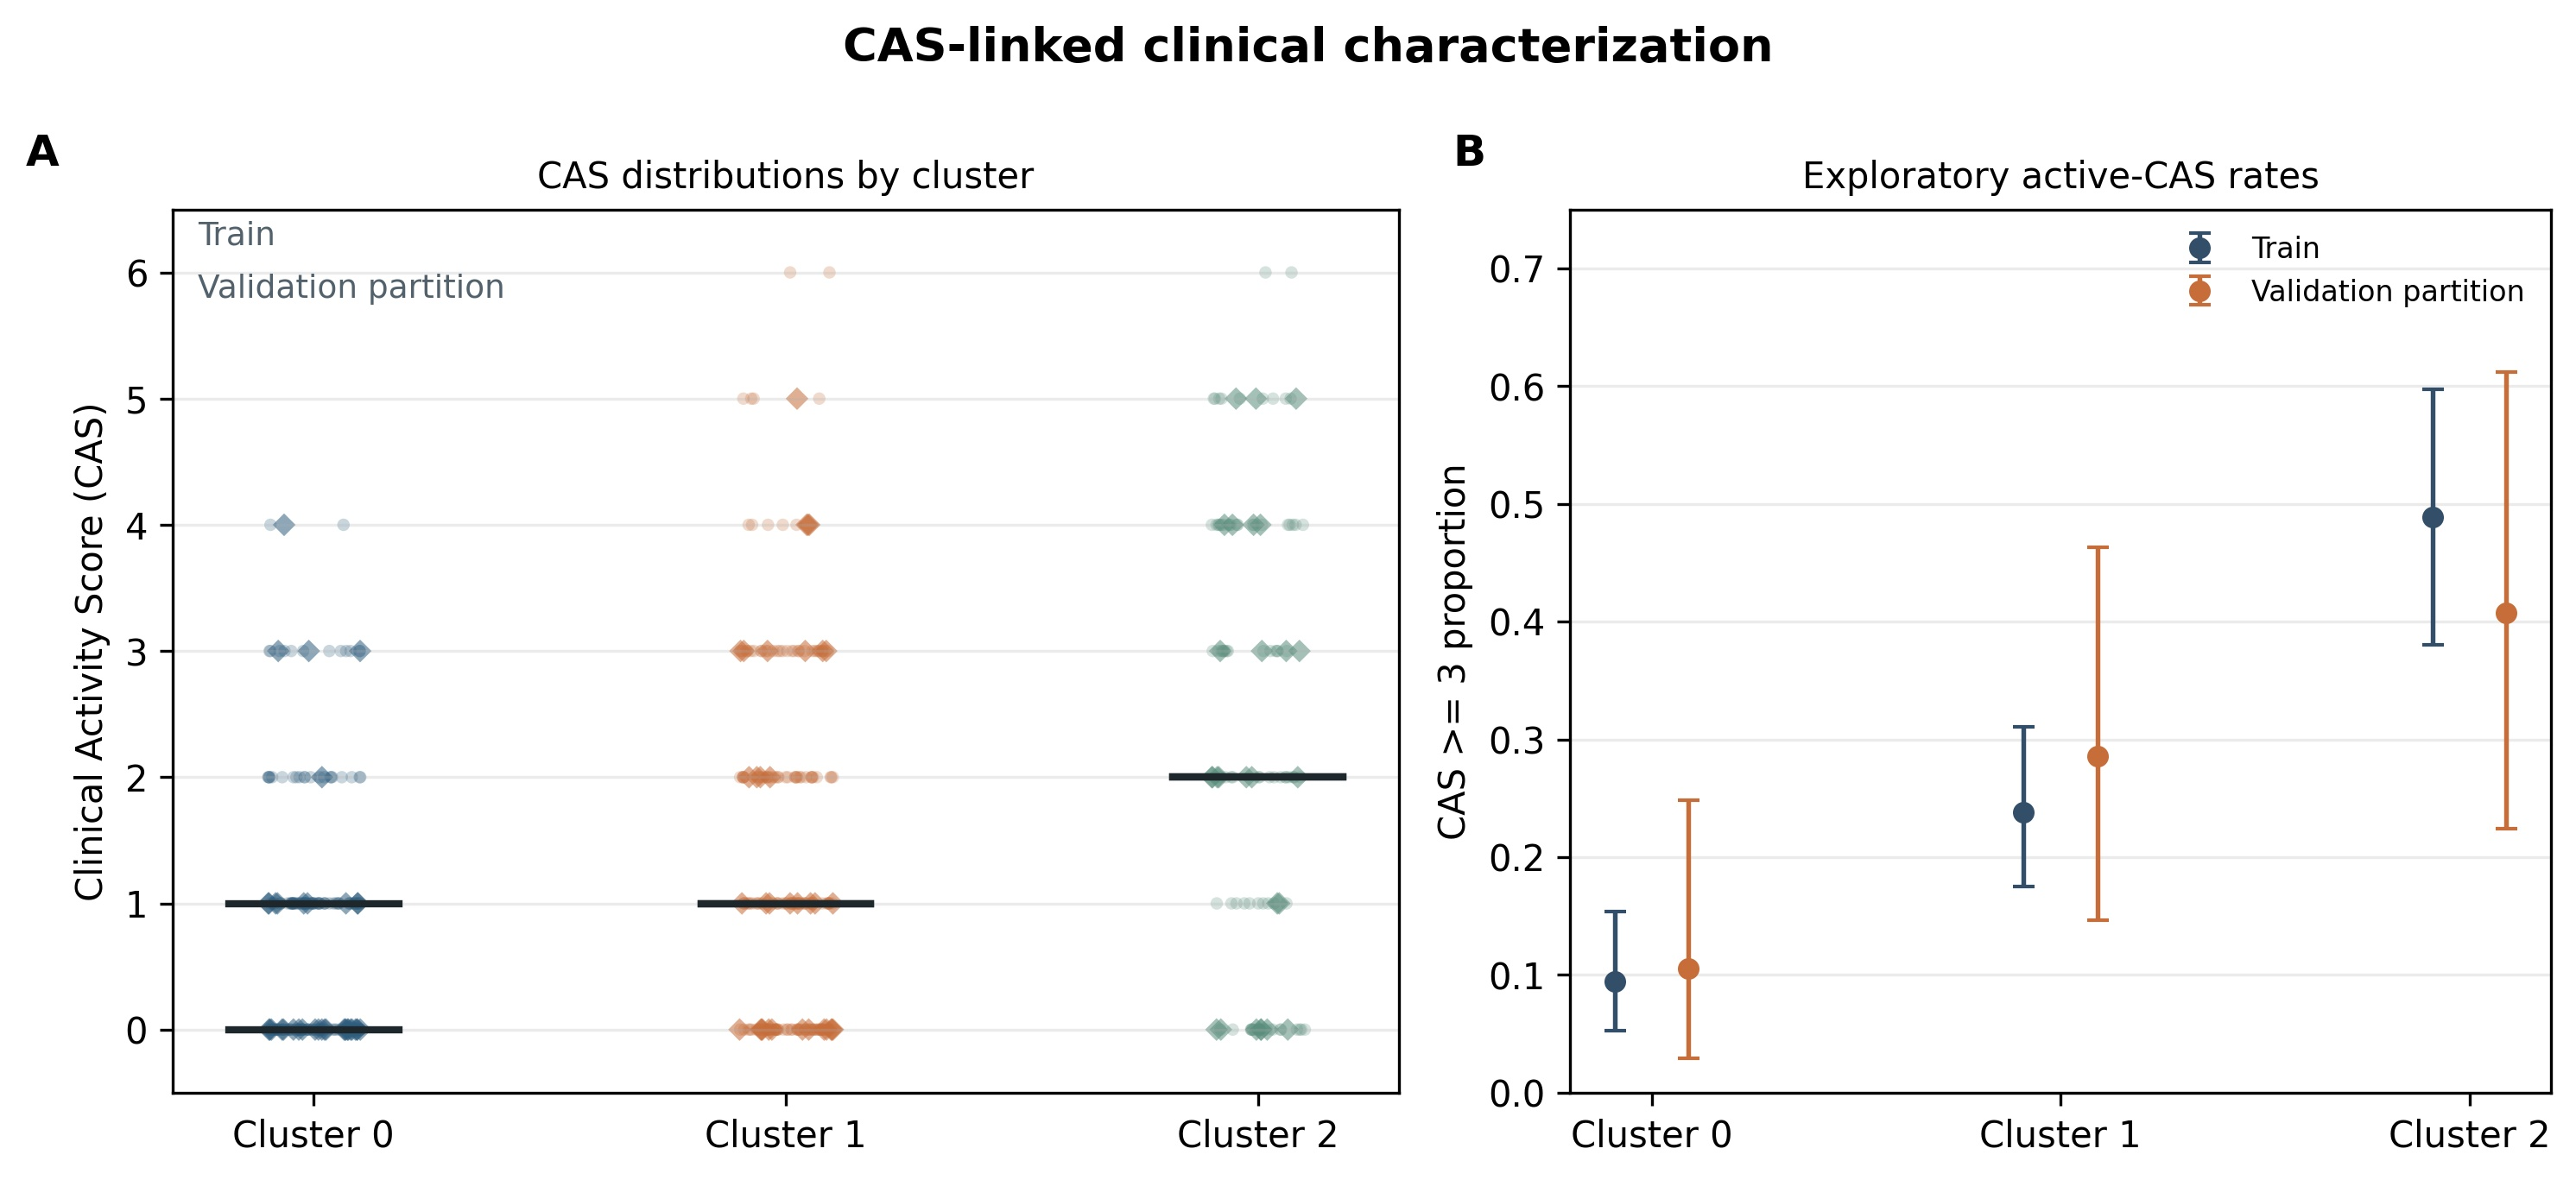
\includegraphics{Figure3_cas_characterization.jpg}
  \caption{CAS characterization across the imaging clusters. The 100 cases shown in the right-hand panels are a fixed validation partition from TOM500, not an independent external cohort.}
  \label{fig:cas}
\end{figure}

\subsection{Covariate-adjusted associations}
Among the 396 complete training cases, the adjusted models showed a graded association between cluster membership and CAS after accounting for age, sex, smoking index, and disease duration. Relative to cluster 0, the adjusted continuous-CAS differences were 0.37 (95\% CI 0.08--0.67) for cluster 1 and 1.19 (95\% CI 0.77--1.61) for cluster 2, with an overall Wald $P=2.09\times10^{-7}$. For CAS $\geq3$, the corresponding odds ratios were 2.42 (95\% CI 1.20--4.87) and 6.55 (95\% CI 3.11--13.79), with an overall Wald $P=2.09\times10^{-6}$. The higher cluster 2 estimate was observed for both endpoint definitions in training.

The 100-case fixed validation partition produced less consistent adjusted evidence. The overall continuous-CAS model had $P=0.0495$. The cluster 1 versus cluster 0 difference was 0.49 (95\% CI $-0.20$ to 1.19), whereas the cluster 2 versus cluster 0 difference was 1.08 (95\% CI 0.20--1.95). For CAS $\geq3$, the overall model had $P=0.543$, with odds ratios of 1.88 (95\% CI 0.47--7.48) for cluster 1 and 2.41 (95\% CI 0.49--11.89) for cluster 2. The continuous endpoint therefore retained nominal overall support, but the binary endpoint did not, and the cluster-specific intervals were wide in the smaller partition. The validation results provide an exploratory internal association signal rather than consistent replication of an adjusted activity association (Figure~\ref{fig:robust}; Table~\ref{tab:adjusted}).

The ordinal sensitivity model showed the same direction of increasing odds with cluster number, but the proportional-odds assessment was constrained by sparse high-CAS categories. In training, common odds ratios were 1.51 (95\% CI 0.98--2.32; $P=0.063$) for cluster 1 and 4.27 (95\% CI 2.45--7.44; $P=2.93\times10^{-7}$) for cluster 2, with an overall Wald $P=1.38\times10^{-6}$. In validation, the corresponding odds ratios were 2.22 (95\% CI 0.84--5.88; $P=0.107$) and 4.40 (95\% CI 1.42--13.64; $P=0.010$), with an overall Wald $P=0.0366$. Threshold-specific fits at CAS $\geq5$ and CAS $\geq6$ did not converge in training because only 16 and 4 cases contributed to those thresholds, and the CAS $\geq5$ fit did not converge in validation because only 4 cases were positive. The ordinal model consequently serves as a sensitivity description of the CAS gradient, while the continuous and binary endpoint results remain the primary adjusted evidence (Table~\ref{tab:ordinal}).

\begin{figure}
  \centering
  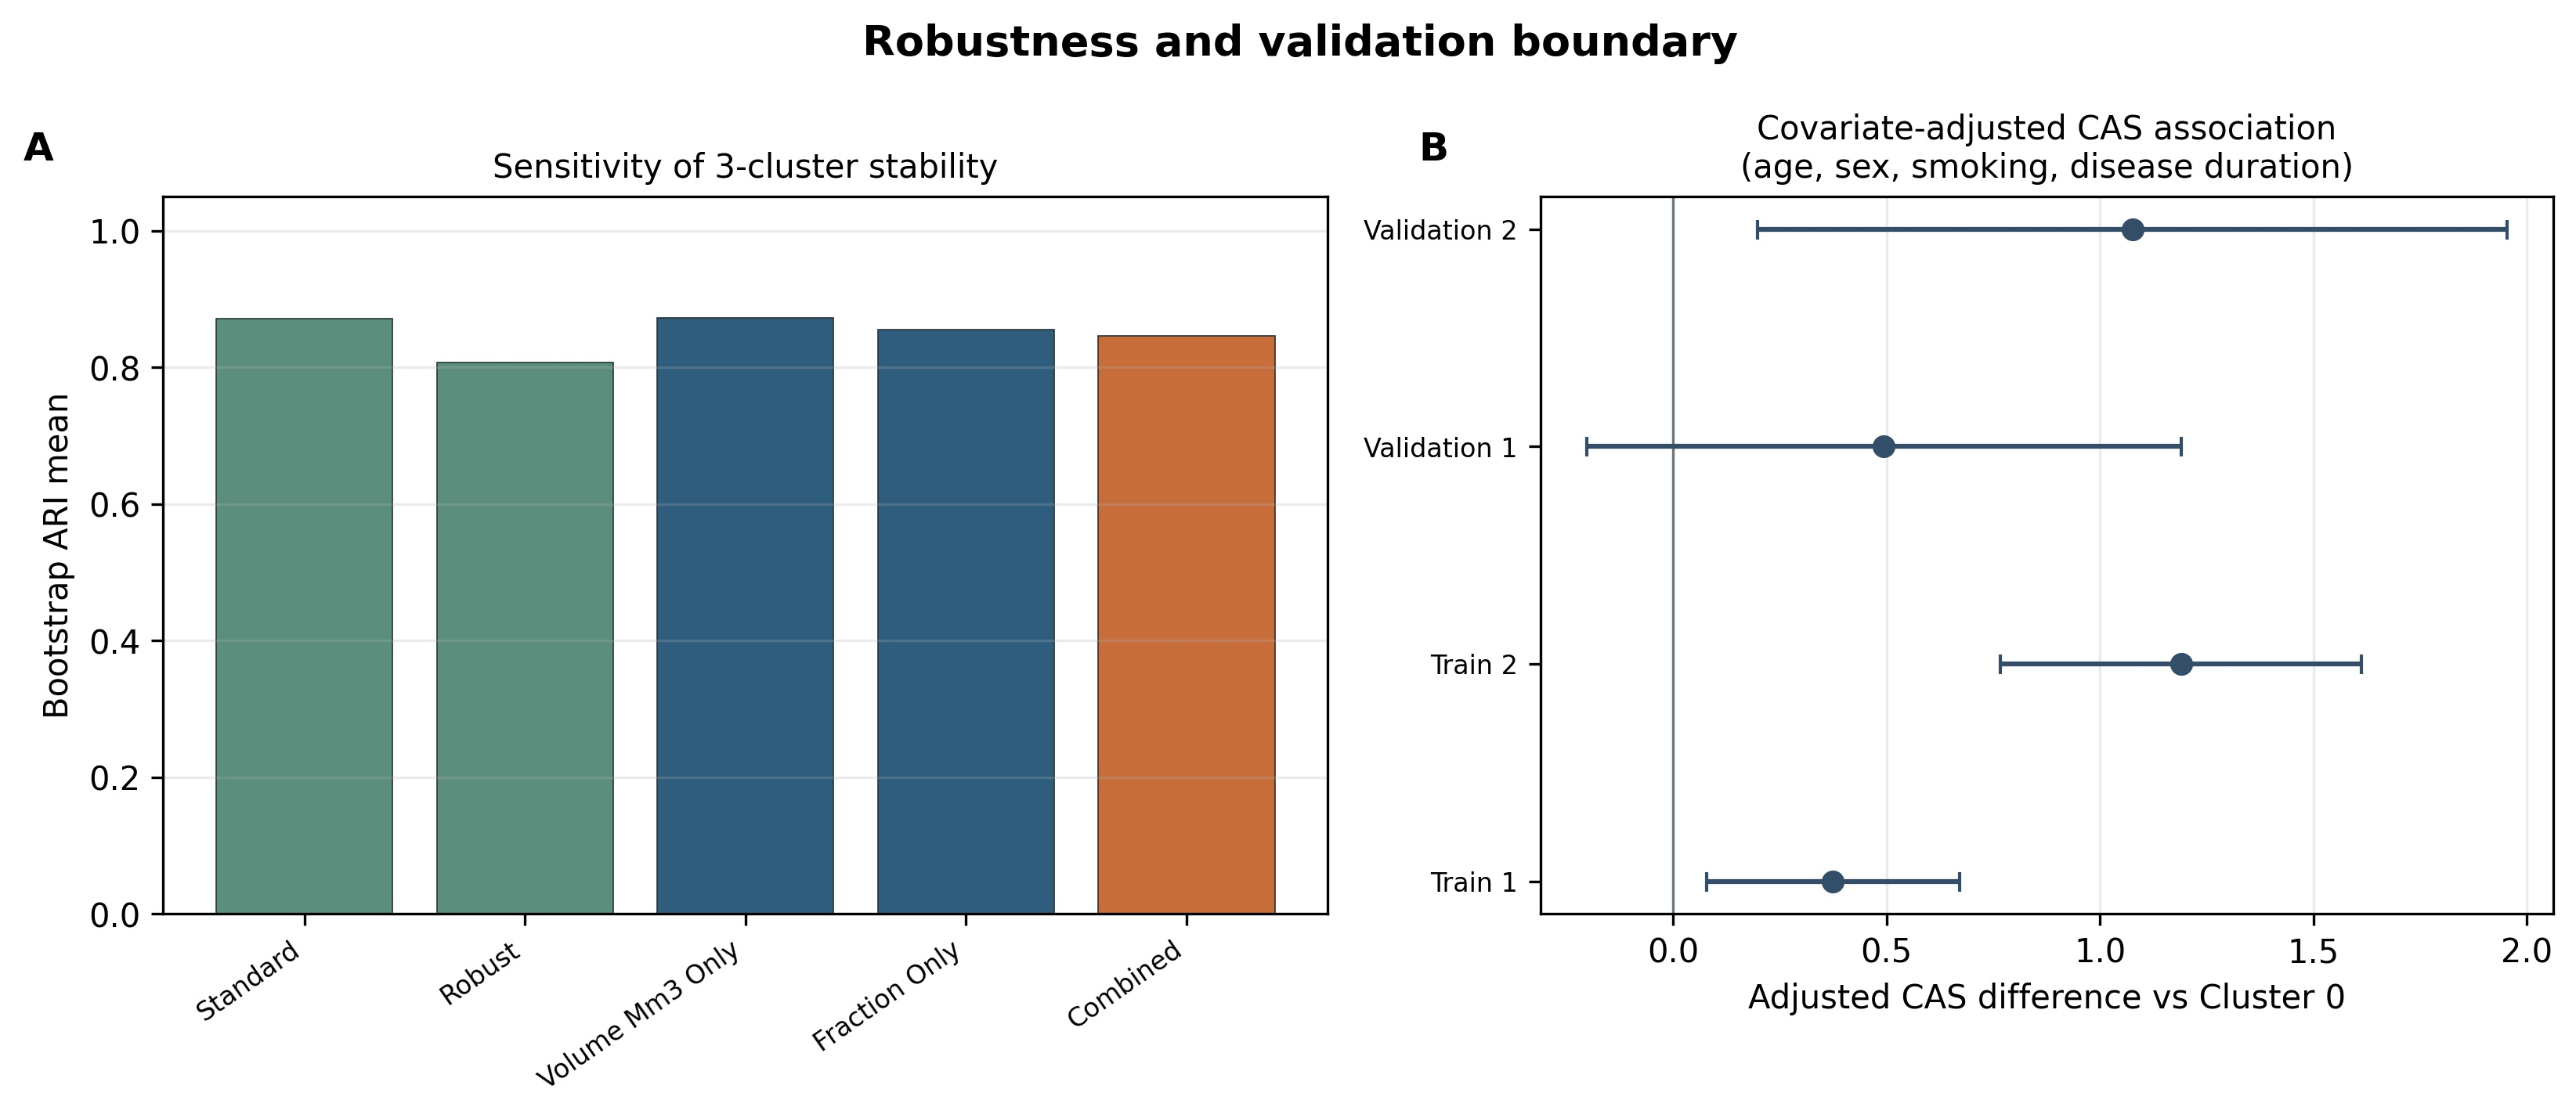
\includegraphics{Figure4_robustness_adjustment.jpg}
  \caption{Robustness and covariate-adjusted association. Sensitivity analyses are shown with ARI relative to the primary solution. The adjusted CAS association attenuated in the fixed validation partition, and this panel is not evidence of independent external validation.}
  \label{fig:robust}
\end{figure}

\begin{table}
\centering
\caption{Covariate-adjusted associations between imaging cluster and CAS. Cluster 0 was the reference. Models adjusted for age, sex, smoking index, and disease duration.}
\label{tab:adjusted}
\scriptsize
\begin{tabular}{llrrrrr}
\toprule
Partition & Outcome & Contrast & Estimate & 95\% CI low & 95\% CI high & $P$\\
\midrule
Training & Continuous CAS & Cluster 1 vs 0 & 0.37 & 0.08 & 0.67 & 0.0131\\
Training & Continuous CAS & Cluster 2 vs 0 & 1.19 & 0.77 & 1.61 & $3.47\times10^{-8}$\\
Training & CAS $\geq3$ & Cluster 1 vs 0 & OR 2.42 & 1.20 & 4.87 & 0.0132\\
Training & CAS $\geq3$ & Cluster 2 vs 0 & OR 6.55 & 3.11 & 13.79 & $7.30\times10^{-7}$\\
Validation & Continuous CAS & Cluster 1 vs 0 & 0.49 & $-0.20$ & 1.19 & 0.165\\
Validation & Continuous CAS & Cluster 2 vs 0 & 1.08 & 0.20 & 1.95 & 0.0163\\
Validation & CAS $\geq3$ & Cluster 1 vs 0 & OR 1.88 & 0.47 & 7.48 & 0.372\\
Validation & CAS $\geq3$ & Cluster 2 vs 0 & OR 2.41 & 0.49 & 11.89 & 0.280\\
\bottomrule
\end{tabular}
\end{table}

\begin{table}
\centering
\caption{Ordinal logistic sensitivity analysis for CAS. Cluster 0 was the reference. Models adjusted for age, sex, smoking index, and disease duration.}
\label{tab:ordinal}
\scriptsize
\begin{tabular}{lrrccc}
\toprule
Partition & $n$ & Contrast & Common OR & 95\% CI & $P$ \\
\midrule
Training & 396 & Cluster 1 vs 0 & 1.51 & 0.98--2.32 & 0.063 \\
Training & 396 & Cluster 2 vs 0 & 4.27 & 2.45--7.44 & $2.93\times10^{-7}$ \\
Validation & 100 & Cluster 1 vs 0 & 2.22 & 0.84--5.88 & 0.107 \\
Validation & 100 & Cluster 2 vs 0 & 4.40 & 1.42--13.64 & 0.010 \\
\midrule
\multicolumn{6}{l}{Overall Wald $P$: training $1.38\times10^{-6}$, validation $0.0366$.}\\
\bottomrule
\end{tabular}
\end{table}

\begin{table}
\centering
\caption{Sensitivity of the three-cluster volume-led phenotype. ARI values compare each sensitivity solution with the primary training solution.}
\label{tab:sensitivity}
\small
\begin{tabular}{lrrr}
\toprule
Analysis & ARI to primary & Bootstrap ARI mean & Validation CAS $P$\\
\midrule
Standard scaling & 1.000 & 0.862 & 0.000401\\
Robust scaling & 0.606 & 0.807 & 0.000216\\
Physical volume only & 0.520 & 0.860 & 0.001683\\
Volume fraction only & 0.761 & 0.861 & 0.002975\\
Combined volume and intensity & 0.270 & 0.847 & 0.001086\\
Leave out one tissue, range & 0.653--0.925 & - & -\\
Single-tissue solutions, range & 0.036--0.316 & - & -\\
\bottomrule
\end{tabular}
\end{table}

\section{Discussion}
The central finding is that a volume-led representation of nine annotated orbital tissues yielded a reproducible exploratory phenotype in TOM500. This result concerns the organization of the imaging data rather than the discovery of a new clinical category. Stability under patient-level resampling, alternative scaling, and tissue deletion indicates that the partition was not generated by a single resampling realization or by one isolated tissue measurement. The poor agreement of single-tissue solutions with the primary partition further supports a coordinated representation of orbital involvement. At the same time, the lower silhouette of the three-cluster solution than the two-cluster solution shows that geometric compactness and reproducibility answer different questions. The present phenotype is therefore best understood as a stable description of heterogeneity under the stated feature and clustering protocol, rather than as a definitive taxonomy of TAO.

The CAS findings provide clinical characterization of this imaging organization, but they do not change its exploratory status. The unadjusted CAS gradient had the same direction after frozen-centroid assignment in the training and fixed validation partitions, which supports a reproducible association signal at the level of clinical characterization. The clusters also differed in age, sex, and smoking index. Those imbalances matter because the same clinical factors can be related to both orbital tissue burden and CAS, so an unadjusted gradient cannot be interpreted as an imaging-specific activity effect. Covariate adjustment retained an association in training, while the fixed validation results differed by endpoint. The continuous CAS model retained nominal overall support, whereas the CAS threshold model did not, and the cluster-specific intervals were imprecise. The ordinal model preserved the direction of the gradient as a sensitivity description, but sparse high-CAS categories limited threshold-specific assessment. Taken together, the evidence supports an exploratory relationship between the volume phenotype and CAS, while the adjusted association has not achieved consistent replication across endpoints within the held-out partition.

The endocrine-imaging contribution is consequently a measurement framework for studying TAO heterogeneity alongside clinical activity assessment. The volume fractions summarize the relative contribution of the nine annotated tissues, and the patient-level aggregation avoids treating the two eyes of one patient as independent observations. This organization can support future analyses that combine orbital morphology with endocrine variables and treatment trajectories. The current data support neither a biochemical interpretation nor a mechanistic one. TSH, FT4, and TRAb were absent from the verified clinical table, and the dataset also lacked proptosis, treatment exposure, and treatment response. The observed clusters therefore cannot be interpreted as Graves autoimmune injury patterns, treatment strata, or clinically actionable activity states. They also cannot replace CAS or define a threshold for treatment selection. Their present value lies in providing a reproducible imaging representation that can be tested against those outcomes when the required measurements are available.

The study design defines the range of evidence that can be transferred beyond this cohort. The 100-case partition tested assignment of frozen training-derived centroids, so it represents fixed internal validation rather than independent external validation. The public single-cohort design also limits causal interpretation, and the mild heterogeneity in voxel spacing leaves acquisition-related variation as a residual source of uncertainty despite the use of image-specific physical volumes. The restrained feature family is useful for auditability and stability assessment, but it does not establish whether high-dimensional texture features add clinical value. The lower agreement of the combined volume and intensity representation with the primary partition reinforces the need to evaluate added feature families against a frozen reference and an independent outcome, rather than to equate greater feature count with stronger evidence. These boundaries define the current result as hypothesis-generating and prevent the imaging phenotype from being presented as a validated biomarker or treatment-selection model.

The next evidentiary step is adjusted replication in a separate cohort with biochemical and treatment variables recorded at the same patient level. Such a study should preserve the volume-fraction definition, report acquisition and spacing distributions, apply preprocessing parameters without information leakage, and evaluate both continuous CAS and clinically motivated ordinal or binary endpoints. External replication should also test whether the phenotype adds information beyond age, sex, smoking history, disease duration, and routine endocrine measurements. Until that evidence is available, the most defensible interpretation is that TOM500 contains a reproducible multi-tissue orbital MRI phenotype with an exploratory CAS gradient, providing a structured starting point for endocrine-imaging research rather than a clinical decision rule.

\section{Conclusion}
Patient-level volume features from nine annotated orbital tissues yielded a reproducible exploratory phenotype in \TOM{}. The three-cluster solution achieved a bootstrap ARI of 0.862 $\pm$ 0.103 across 1,000 training resamples, and single-tissue solutions did not reproduce the multi-tissue organization, with ARI values of 0.036--0.316 relative to the primary partition. The concordant unadjusted CAS gradient after frozen-centroid assignment in the training and fixed validation partitions supports clinical characterization of the phenotype, whereas the inconsistent adjusted validation evidence confines this finding to an exploratory association rather than a validated activity marker. This study establishes an auditable volume-based framework for describing orbital MRI heterogeneity and provides a patient-level foundation for future endocrine-imaging research that integrates biochemical and treatment variables.

\section*{Author contributions}
Cuicui Liu: Methodology, software, formal analysis, visualization, and writing, original draft. Huan Peng: Data curation, validation, and writing, review and editing. Shuang Wu: Supervision, project administration, and writing, review and editing.

\section*{Funding}
The authors received no specific funding for this work.

\section*{Declaration of competing interest}
The authors declare that the research was conducted in the absence of any commercial or financial relationships that could be construed as a potential conflict of interest.

\section*{Ethics approval and consent to participate}
This study used a publicly available, de-identified TOM500 dataset and involved no new participant recruitment, intervention, or access to identifiable clinical materials. No additional ethics approval number was required for this secondary analysis of the public resource.

\section*{Consent to publish}
This study used a publicly available, de-identified dataset and did not include identifiable individual information requiring publication consent.

\section*{Data availability}
The TOM500 dataset analyzed in this study is publicly available through Figshare at DOI \href{https://doi.org/10.6084/m9.figshare.27133389}{10.6084/m9.figshare.27133389}, subject to the repository's access and citation conditions. Derived feature tables and result files are available from the corresponding author upon reasonable request.

\section*{Code availability}
The analysis code used to generate the reported feature tables, clustering analyses, sensitivity analyses, adjusted associations, and figures is available at the public repository \href{https://github.com/Hajimi-Sudo/tom500-orbital-mri-phenotyping}{https://github.com/Hajimi-Sudo/tom500-orbital-mri-phenotyping}. Raw MRI files, masks, patient-level derived tables, and access credentials are not included in the repository.

\section*{Acknowledgements}
The authors acknowledge the TOM500 dataset contributors for making the de-identified imaging resource publicly available.

\bibliographystyle{Frontiers-Vancouver}
\bibliography{references}

\end{document}
